
%
%  $Description: Author guidelines and sample document in LaTeX 2.09$ 
%
%  $Author: John Burchell & William Granli $
%  $Date: 2015/01/21 15:20:59 $
%  $Revision: 1.0
%

\documentclass[10pt,twocolumn]{article} 
\usepackage{latex8}
\usepackage{url}
\usepackage{verbatim}
\usepackage{fixltx2e}
\usepackage{graphicx}
%\documentstyle[times,art10,twocolumn,latex8]{article}

%------------------------------------------------------------------------- 
% take the % away on next line to produce the final camera-ready version 
\pagestyle{empty}

%------------------------------------------------------------------------- 
\begin{document}



\title{Assignment 4}

% author names and affiliations
\author{John Burchell and William Granli \\
john.a.burchell, william.granli@gmail.com}


\maketitle
\thispagestyle{empty}

%------------------------------------------------------------------------- 


\Section{Methodology}
This section will describe which statistical tests were used, and why. The level of significance used for all tests is 5\%. 

\SubSection{Tests Used for H\textsubscript{eff} and H\textsubscript{rate}}
Initially, Kolmogorov-Smirnov (KS) Goodness-of-Fit and Shapiro-Wilks (SW) tests were used to determine if the assumption of normality could be held for the data set. The KS and SW tests both reported p-values < 0.05 and thus the null hypotheses of the data being normally distributed was rejected. See Table 1 for the results of the KS and SW tests. 

\begin{table}
	\centering
	\begin{tabular}[ht]{| l | l | l |}
	\hline
	Test & Sample & p-value  \\
	\hline
	KS & UC & =< 2.2e-16 \\
	\hline
	SW & UC & 0.000969 \\
	\hline
	KS & CL & =< 2.2e-16 \\
	\hline
	SW & CL & 0.309 \\	
	\hline
	\end{tabular}
	\caption{Results of normality tests}
\end{table}

A graphical representation of the level of normalisation can be seen in Figure 1 and 2. The results from the tests are supported by the sparseness of the data points. 

\begin{figure}[Ht!]
\centering
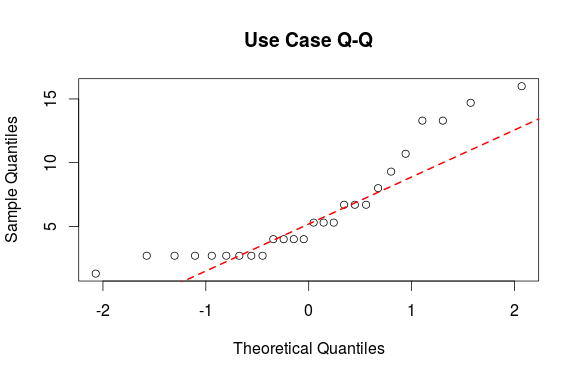
\includegraphics[width=90mm]{uc_qq.png}
\caption{Use Case Q-Q plot}
\end{figure}

\begin{figure}[Ht!]
\centering
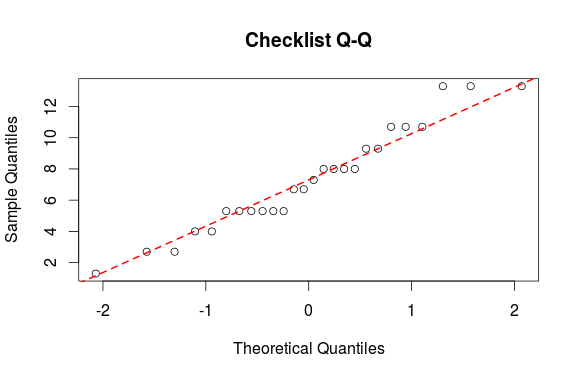
\includegraphics[width=90mm]{cl_qq.png}
\caption{Checklist Q-Q plot}
\end{figure}


The next step was to perform outlier test. The method used was boxplots. As seen in Figure 3 and 4, no outliers were detected and thus no data points were removed in the tests performed. 

\begin{figure}[Ht!]
\centering
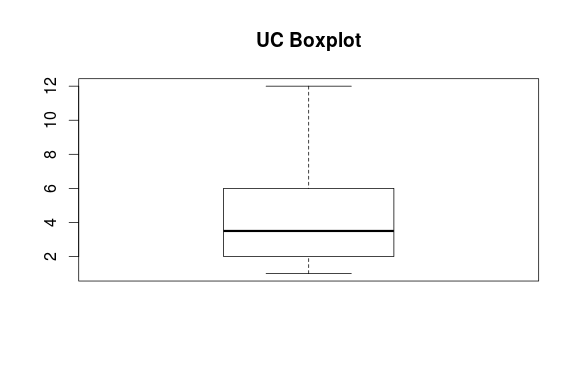
\includegraphics[width=90mm]{uc_box.png}
\caption{Use Case Boxplot}
\end{figure}

\begin{figure}[Ht!]
\centering
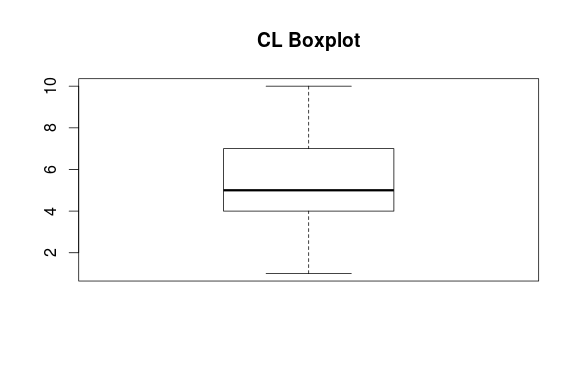
\includegraphics[width=90mm]{cl_box.png}
\caption{Checklist Boxplot}
\end{figure}

Since the data is non-normalised, the Wilcoxon-Mann-Whitney (WMW) two-sample rank-sum teset was chosen instead of the Student's T-test as the final test. The result of the WMW test was W=250, p=0.1063 and with the significance level of 89 (cite www.sussex) H0 is rejected. (Note that this was done on the raw data and not /45*60).


http://www.sussex.ac.uk/Users/grahamh/RM1web/WilcoxonTable2005.pdf



MWW = good for cont tests as well.
 Mann, Henry B.; Whitney, Donald R. (1947). "On a Test of Whether one of Two Random Variables is Stochastically Larger than the Other". Annals of Mathematical Statistics 18 (1): 50–60. doi:10.1214/aoms/1177730491. MR 22058. Zbl 0041.26103.

1 and 2.
Box
->
Histo, QQ, kolmogorov, z-test?
->
T

3.
Z-test verkar vara ett alternativ till chi

* Method(s) for analyzing the data (Statistical analysis)

* Motivation of why these statistical tests where used

\Section{Results}

*Report the results

*Discuss what does the results means, how do we interpret it

\Section{Tests for eff}

\verbatiminput{f_eff.txt}

Since the p-value is larger than 0.05, we can deduce that the variances are homogeneous (cite expe) and that the T-test is the optimal approach.

\verbatiminput{t_eff.txt}

According to the test, the efficiency of CL is 7.3 while the efficiency of UC is 6.16 and H0 eff is therefore rejected. 

\Section{Tests for rate}

\verbatiminput{f_rate.txt}



Since the p-value is larger than 0.05, we can deduce that the variances are homogeneous (cite expe) and that the T-test is the optimal approach.


\verbatiminput{t_rate.txt}

According to the test, the rate of CL is 1.45 while the effectiveness of UC is 0.12 and h0 rate is therefore rejected. 

\Section{Tests for 3}

%%R output
	Chi-squared test for given probabilities

data:  ct
X-squared = 5.4847, df = 2, p-value = 0.06442

Since our significance level is 0.05 and p > 0.05, there is no significant difference and h1 is rejected. 
%%R output


Chi-square test requirements[edit]
Quantitative data.
One or more categories.
Independent observations.
Adequate sample size (at least 10).
Simple random sample.
Data in frequency form.
All observations must be used.
\bibliographystyle{latex8}
\bibliography{latex8}


\Section{Acknowledgements}
U w0T m8


\end{document}

